
% ----------------------------- %
% Section 1
% ----------------------------- %
\section*{Solution}
The first thing that comes to my mind
when I look at this problem is that
the numerator can be factored into
$ (\theta + 3)(\theta + 2) $ which
means our problem becomes
\begin{equation}
	\textbf{33.}\quad \int_{-1}^{\infty} 
	\frac{d\theta}{\theta^2+5\theta+6}
	=
	\int_{-1}^{\infty} 
	\frac{d\theta}{(\theta + 3)(\theta + 2)}	
\end{equation}

After that, we can use partial fraction decomposition
to make the integrand easier to integrate.
\begin{equation}
	\int_{-1}^{\infty} 
	\frac{d\theta}{(\theta + 3)(\theta + 2)}
	=
	\int_{-1}^{\infty} 
	\frac{A}{\theta + 3} + \frac{B}{\theta + 2} d\theta
\end{equation}

We can then multiply both sides of the
equation with $ (\theta + 3)(\theta + 2) $.
For the sake of readability, let's 
skip the integral notation for now
and look at only the coefficients now.
\begin{align}
	1
	&=
	A(\theta + 2) + B(\theta + 3) \\
	(0)\theta + (1)
	&=
	(A+B)\theta + (3A + 2B)
\end{align}

Solving for these two equations
$ A + B = 0 $ and 
$ 3A + 2B = 1 $ gives us
\begin{align}
	A &= 1 \\
	B &= -1
\end{align}

In other words, if we put everything 
back to the original equation together,
we get something that's much more easier
to integrate: 
\begin{equation*}
	\int_{-1}^{\infty} 
	\frac{d\theta}{(\theta + 3)(\theta + 2)}
	=
	\int_{-1}^{\infty} 
	\frac{1}{\theta + 3} + \frac{-1}{\theta + 2} d\theta
\end{equation*}

\newpage

Well, why is it easier to integrate?
It's because 
$ \int \frac{1}{x} $ is elegantly
$ ln|x| + C $.
\begin{align}
	\int_{-1}^{\infty} 
	\frac{d\theta}{(\theta + 3)(\theta + 2)}
	&=
	\Bigl[
	ln|\theta + 2| - 
	ln|\theta + 3| + C
	\Bigr]_{-1}^{\infty} \\
	&=
	\Big[
	0
	\Big]
	-
	\Big[
	-ln2
	\Big] \\
	&=
	ln2
\end{align}






\begin{comment} 


% ----------------------------- %
% Section 2
% ----------------------------- %
\section*{Verifying the Integral}

\begin{figure}
	\centering
	\caption[Figure 1. The integrand and the integral.]{}
	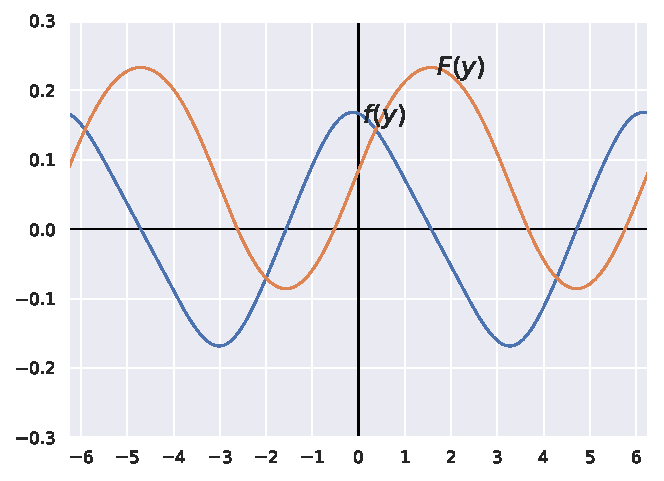
\includegraphics[width=0.7\linewidth]{graph_1}
	\label{fig:graph1}
\end{figure}

Let's see if we got the correct integral
by graphing it. One thing I've noticed
from this graph is that whenever $ f(y) $ is at $ 0 $, 
$ F(y) $ is either at its minimum or maximum.
For instance, at $ f(y) \approx -1.6 $,
$F(y)$ is at its minimum.
Notice that this is one of the properties we learned
in Calculus I. 

The integrand
of our original problem $ f(y) $ seems to be the
derivative of the integral we got, which is $ F(y) $.

\end{comment}